\section{context}
Binnen de wereld van competitieve sporten en evenementen, zoals marathons, wielerrondes en rallyraces, zijn nauwkeurige tijd en plaatsbepaling noodzakelijk. Tegenwoordig wordt er bij moderne analyses en live tracking verwacht dat er continu een accurate positiebepaling van de deelnemers plaatsvindt. Wedstrijden hangen namelijk vaak af van fracties van seconden en centimeters. In dit hoofstuk wordt dan ook de nadruk gelegd op het huidige systeem en zijn beperkingen.


\subsection{GNSS}

De basis voor moderne positiebepaling wordt gevormd door Global Navigation Satellite Systems (GNSS), de overkoepelende term voor systemen zoals het Amerikaanse GPS en het Europese Galileo. In de kern functioneert GNSS doormiddel van timing \cite{GNSSConstellations2026}. De ontvanger berekent zijn positie door de exacte reistijd van signalen tussen de satellieten en de antenne te meten. Om een betrouwbare driedimensionale positie te bepalen, is verbinding met minimaal vier satellieten vereist \cite{novatel_computation}. Dit minimum is noodzakelijk om de vier onbekende variabelen op te lossen: de breedtegraad, lengtegraad, hoogte en de tijdsafwijking van de receiver clock. Hoe meer satellieten daarbovenop worden meegenomen, hoe nauwkeuriger de uitkomst zal zijn. Omdat radiosignalen zich met de lichtsnelheid verplaatsen, is die nauwkeurige tijdmeting en synchronisatie noodzakelijk, aangezien de afstand direct af te leiden is uit de verstreken tijd. \\

Hoewel GNSS-ontvangers breed inzetbaar zijn, kent deze techniek beperkingen. Een standaard smartphone-GPS behaalt onder ideale omstandigheden een nauwkeurigheid van grofweg 4,9 meter \cite{gpsgov2026accuracy}. Voor het nauwkeurig volgen van een atleet of voertuig op een wedstrijdparcours is deze foutmarge vaak onacceptabel groot.


\subsection{Nauwkeurigheid via RTK}
Om deze beperkingen te overkomen, wordt gebruikgemaakt van Real Time Kinematic (RTK). Dit systeem bestaat uit twee ontvangers, namelijk een stationair 'Base Station' op een bekende locatie en een mobiele 'Rover Receiver' \cite{gpsgeometer_rtk}. Het basisstation berekent de afwijkingen in het satellietsignaal die worden veroorzaakt door clock errors en vertragingen in de atmosfeer. Deze correcties worden verstuurd naar de Rover, waardoor een theoretische nauwkeurigheid van minder dan 50 mm behaald kan worden \cite{valente2020accuracy}.


\subsection{Gebreken}
De hoge nauwkeurigheid is in de praktijk sterk afhankelijk van de omgeving. Omdat GNSS gebasseerd is op de aankomsttijd van signalen, is het systeem kwetsbaar voor signaalreflecties en blokkades \cite{NovAtelMultipath2026}. Hieronder zijn dan ook een aantal prominente fouten die relevant zijn kijkend naar GNSS:

\begin{enumerate}
    \item \textbf{Non Line of Sight (NLOS):} De directe zichtlijn naar de satelliet is geblokkeerd. Het gebruik van RTK helpt hierbij aangezien het meestal gebruik maakt van een 'base' van een zeker hoogte om zo objecten te vermijden.
    \item \textbf{Multipath effecten:} Het signaal weerkaatst tegen een object voordat het de antenne bereikt. Hierdoor legt het signaal een langere weg af en komt het later aan. De ontvanger interpreteert deze extra reistijd onterecht als een grotere afstand tot de satelliet, wat resulteert in een positiefout. Dit is dan ook in recent onderzoek naar robuuste lokalisatie van Yuming Yin \cite{pmc_sensorfusion} aangetoont. Hieruit blijkt dat in dergelijke situaties de maximale precisie niet behouden kan worden.
    \item \textbf{Satelliet klok:} De GNSS satellieten bevatten atoom klokken die zeer nauwkeurig zijn, maar toch kunnen afwijken. Een afwijking van 10 ns kan resulteren in een fout van 3 meter \cite{NovAtelGNSSerrorSources2026}. Om hiervoor te compenseren kan er zeer nauwkeurige klok informatie van een Space Based Augmentation System (SBAS) of Precise Point Positioning (PPP) service provider gedownload worden. Dit bevat correcties voor deze afwijkingen die berekend worden door de SBAS of PPP. Hiernaast is het gebruken van RTK een goede oplossing.
    \item \textbf{Baanafwijkingen:} Naast het feit dat de klok kan afwijken, is dit ook het geval wanneer er gekeken wordt naar het traject die de satelliet aflegt. Hierbij is RTK een goede oplossing.
    \item \textbf{Ionospheric delay:} De ionosfeer is een laag in de atmosfeer die zich tussen de 50 en 1000 km boven aarde bevindt. De ionen die zich hierin bevinden beïnvloeden de transmissie tijd van de satelliet signalen. Aangezien deze condities in een lokaal gebied vrij gelijk zijn, zullen zowel de receiver als de base station van de RTK een vergelijkbare vertraging meemaken. Hiervoor kan dan ook gecompenseert worden.
    \item \textbf{Tropospheric delay:} Dit is de laag in de atmosfeer die het dichtstbij de aarde ligt. Hierbij ontstaat vertraging door verandering in temperatuur, luchtvochtigheid en druk. Ook hier kan de RTK voor compenseren aangezien deze condities vrij constant zijn in het te meten gebied.
\end{enumerate}

De multipath en NLOS effecten zijn uitgebeeld in figuur \ref{fig:multipath}. Bovendien zijn de afwijkingen aangetoond in tabel \ref{tab:gnss_error_sources}.


\begin{figure}[htbp!]
    \centering
    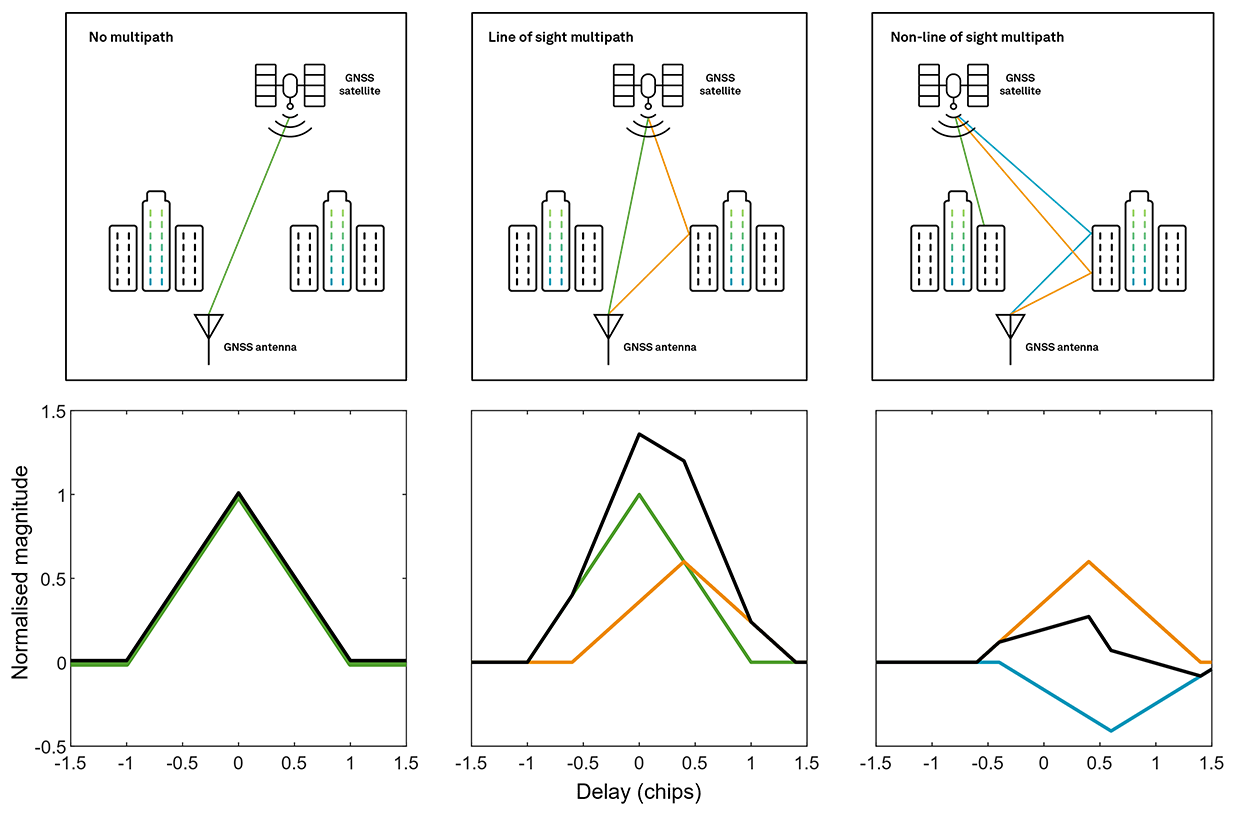
\includegraphics[width=0.8\linewidth]{images/multipath voorbeeld.png}
    \caption{In de afbeelding is het effect van zowel multipath als non line of sight in statistieken uiteengezet. De groene lijn staat voor het directe signaal, en de gele en blauwe staan voor de multipath signalen. De zwarte lijn is wat de ontvanger waarneemt \cite{NovAtelMultipath2026}}
    \label{fig:multipath}
\end{figure}


\begin{table}[h]
    \centering
    \caption{Belangrijkste GNSS foutbronnen en hun typische foutbereik \cite{NovAtelMultipath2026}}
    \label{tab:gnss_error_sources}
    \begin{tabular}{l c}
    \hline
    \textbf{Foutbron} & \textbf{Typisch foutbereik} \\
    \hline
    Multipath & $\pm 1$ m \\
    Satelliet klok & $\pm 2$ m \\
    Baanafwijkingen & $\pm 2.5$ m \\
    Ionospheric delays & $\pm 5$ m \\
    Tropospheric delays & $\pm 0.5$ m \\
    \hline
    \end{tabular}
\end{table}

\newpage


\subsection{Sensor Fusion}
Om deze beperkingen aan te pakken, wordt voornamelijk gekeken naar de sensorfusie van de IMU, aangezien dit een van de meest prominente oplossingen is. Een IMU werkt autonoom en is daardoor ongevoelig voor externe storingen of signaalblokkades. Door de data van de accelerometer en gyroscoop in de tijd te integreren, kan de IMU continu een complete navigatiestatus (positie, snelheid en oriëntatie) leveren. \\

De noodzaak om deze sensoren te combineren is gebaseerd op het feit dat ze elkaar nuttig aanvullen.
Waar een alleenstaande IMU lijdt aan oplopende drift waardoor de positienauwkeurigheid na verloop van tijd verslechterd, biedt GNSS juist positiebepaling zonder drift. Door beide systemen te combineren, ontstaat er een robuuste oplossing. De IMU blijft de positie schatten wanneer GNSS wegvalt of onbetrouwbaar is door obstakels, terwijl de GNSS metingen worden gebruikt om de drift van de IMU te corrigeren en de fouten te beperken. \\
 
Bij het combineren van deze twee systemen komt meer kijken dan alleen het vergelijken van de data met elkaar. Een veel voorkomend algoritme hiervoor is de Extended Kalman Filter (EKF). Dit is belangrijk aangezien bewegingsmodellen zelden lineair zijn. Het EKF algoritme lost dit op door niet lineaire systeemdynamiek lineair te maken en te benaderen rondom de huidige staatsschatting (current state estimates) \cite{Meng2017RobustLocalization}. Hiermee kan, ondanks de ruis in de metingen, toch een optimale schatting van de positie gemaakt worden.



\begin{itemize}
    \item \textbf{IMU:}
    \item \textbf{}
\end{itemize}








\newpage